\documentclass[a4paper]{article}
\usepackage[margin=1in]{geometry}
\usepackage[english]{babel}
\usepackage[utf8]{inputenc}
\usepackage{amsmath}
\usepackage{graphicx}
\usepackage[colorinlistoftodos]{todonotes}

\title{Spreadsheet Error Detection with a Type System}

\author{You}

\date{\today}

\begin{document}
\maketitle


\section{Motivation}
According to U.S. Bureau of Labor and Statistics, there will be fewer than 3 million professional programmers, but more than 55 million people using spreadsheets and databases at work by 2012~\cite{scaffidi2005}. Despite the popularity of spreadsheet programming, the lack of training of these non-professional end-user programmers leads to many errors in business spreadsheets that on average the cell error rate is 3.9\%~\cite{panko2016we}. These errors cost great loss.

Spreadsheet errors fall in to three categories: logical errors (45\%), mechanical errors (23\%), and omission errors (31\%). Logical errors cover the most part and the main reasons account for logical errors are mathematical and domain knowledge. Mechanical errors refer to the cases in which wrong cells are pointed at or typing errors occurs. Omission errors is similar to mechanical errors which happens due to the cases that leaves out necessary components. Because of the complex dependency in spreadsheet programming, these errors are hard to be detected or fixed clearly through manual check.

In our study, we are interested in how to detect the mechanical errors, omission errors and part of logical errors in spreadsheet using static analysis techniques, like type system? 

\section{Method}
In this section, we will detail the method for our study.
\subsection{Definition}
\subsubsection{Syntax of spreadsheets}
Note: $e$ is expression, $\varepsilon$ is blank cell, $\epsilon$ is error cell, $v$ is value, $a$ is address, $\omega$ is operations, $n$ is the number of parameters required by the operation.
\begin{table}[h]
\centering
\caption{Syntax of spreadsheets}
\begin{tabular}{lll}
\hline
Cell address& : & $a$\\
Cell expression& : & $e$ ::= $\varepsilon | \epsilon | v | a | \omega^{n}(e_1, . . . , e_n)$\\
Spreadsheet&:& $s$ ::= $(a_1, e_1)$ ; . . . ; $(a_m, e_m) i \neq j \Rightarrow a_i \neq a_j$\\
\hline
  \end{tabular}
\label{syntax}
\end{table}

\subsubsection{Basic Types}
Basic Types: Dependent Type, AND Type, and OR Type.
\begin{figure}[!tb]
\centering
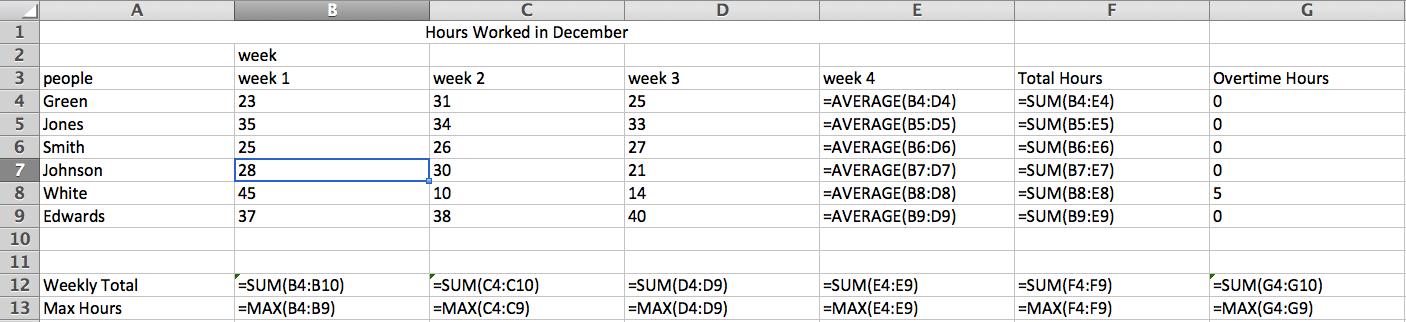
\includegraphics[width=1\columnwidth]{formula.png}
\caption{An example from corpus in formula view}
\label{sheet}
\end{figure}

\begin{itemize}
\item Dependent Type: Cells with value $v$ and header $t$ are in type $t[v]$, e.g. type for cell B3 is \textbf{week[week1]}. It can be recursively defined. e.g. type for cell B7 is \textbf{week[week1[28]]}. 
\item AND Type: Cells with one more types are in type $t1[v]\&t2[v]$, e.g. type for cell B7 is \\
\textbf{week[week1[28]]\&people[Johnson[28]]}.
\item OR Type: Cells with operations referred to other n cells will have a type $t_1[v]|t_2[v]...|t_n[v]$, e.g. type for cell B12 is \\
\textbf{week[week1[23]]\&people[Green[23]] $|$ ... $|$ week[week1[37]]\&people[Edwards[37]]}.
\end{itemize}

\subsubsection{Type Inference Rules}
To 
\subsubsection{Judgments}
\begin{enumerate}
\item Every value that does not have a header is a well-typed.
\item If a cell has value $v$ and header $t$, then it $t[v]$ is well-typed.
\item For AND Type, if there is no common ancestor, it is well-typed. 
\item For OR Type, if there is a common header ancestor, it is well-typed.
\end{enumerate}


\section{Simple Example}
Refer to Figure~\ref{sheet}.
\begin{itemize}
\item By spatial analysis and operational semantics of each formula, we can know the ``type" for each cell. 
\item For cell B12, by spatial analysis, we know that the type is \textbf{WeeklyTotal[193] \& week[week1[193]]}. Since there is no common ancestor of \textbf{WeeklyTotal[193] and week[week1[193]]}, with Judgment 3, we know it is well-typed.
\item For cell B12, by analyzing the operational semantics, we know that the type is \\
\textbf{week[week1[23]]\&people[Green[23]] $|$ ... $|$ week[week1[37]]\&people[Edwards[37]]}. \\
Since there is common ancestor week, thus with Judgment 4, we know it is well-typed.
\item If there is a cell with formula ``A5 + C4", via analysis, we know it is typed as \textbf{people[Jones]$|$week[week2[31]]}.\\ 
Since there is no common ancestor, it is ill-typed and it will be marked as a potential wrong cell.
\end{itemize}

\section{Expectation of Project}
In this section, we will list the expectation output of our study.
\subsection{Implementation}
We are going to implement a type system for spreadsheet error detection. The following are the tools and paper we will refer to.
\begin{enumerate}
\item Parser: http://ewbi.blogs.com/develops/popular/excelformulaparsing.html
\item Type system:
  \begin{enumerate}
	\item basic: \cite{Abraham2006}
    \item advanced: \cite{Cunha2015}
  \end{enumerate}
\item Spatial Analysis:
  \begin{enumerate}
	\item basic: \cite{Abraham2004}
    \item advanced: \cite{Chambers2009a}
  \end{enumerate}
\item Evaluation: We will use the benchmark provided by End-user Spreadsheet Corpus~\cite{fisher2005euses}.
\end{enumerate}

\subsection{Report}
We will report with a survey with all the papers in the bibtex file. We will propose possible improvement based on current implementation in two possible tracks: (1) Extend typing rules with operational semantics of more spreadsheet functions; (2) Automatic error fixing (creating a fixing language (DSL) and do syntactical heuristic search).

\section{Plan}
We will finish the implementation of basic type system and basic spatial analysis by the end of March; and extend the system in proposed direction till the mid of April.
We will focus on report drafting in the left two weeks.

\section{References}

% \bibliographystyle{apacite}
% \bibliography{bibfile}

\end{document}